\documentclass[a4papper, 11pt]{article}

\title{-- Digital Microelectronics --- SoundLoc -- \\ Localication of Soundsources by cross-correlating three $\Sigma\Delta$-microphon signals}
\author{Stefan Kull, Roy Seitz, Marco Zollinger}

\usepackage[T1]{fontenc}			%umlaute als eigene Zeichen
\usepackage[latin1]{inputenc}	%umlaute erkennen
\usepackage{lmodern}
\usepackage{amsmath} 					%mathematischen Textsatz.
\usepackage{amssymb}					%	-Erweiterte math. Sonderzeichen
\usepackage{dsfont}						%	-Mengen			
\usepackage[english]{babel}
\usepackage{textgreek}
\usepackage{siunitx}
\usepackage{graphicx}
\usepackage{caption}			%f�r \captionof

\usepackage[
	pdftitle={SoundLoc -- Digital Microelectronics Project},						%Titel des PDF Dokuments.
	pdfauthor={Stefan Kull, Roy Seitz, Marco Zollinger},									%Autor des PDF Dokuments.
	pdfsubject={Sound localication useing cross correlation of three microphones},		%Thema des PDF Dokuments.
	pdfcreator={LaTeX with hyperref and KOMA-Script},		%Erzeuger des PDF Dokuments.
	pdfkeywords={Cross correlatin, CIC, IP, AXI4\_Lite interface},						%auch f�r PDF Dokumente indexiert
	%	pdfpagemode=UseOutlines,								%Inhaltsverzeichnis anzeigen beim ffnen
	pdfdisplaydoctitle=true,								%Dokumenttitel statt Dateiname anzeigen.
	pdflang=en,												%Sprache des Dokuments.
	plainpages=false,
	hidelinks,												%keine Box um Links
	%	bookmarksopen.											%toc beim �ffnen expandiert
	pdfpagelabels
]{hyperref}

\usepackage[
%includeheadfoot,		%Kopf- und Fusszeilen verwenden
%headheight=15pt,		%H�he der Kopfzeile
left=30mm,				%abstand von Seitenraendern
right=30mm,				%
top=20mm,
bottom=20mm,
%			twoside
]{geometry}



\begin{document}
\maketitle
%\setcounter{tocdepth}{2}
%\tableofcontents

\section{Overview}
\label{sec:overview}

This Document describes the functionality and usage of the XCorr IP core.
It is supplied as a complete, ready to use IP core but without high level software support.
This is due to the project extent which is higher than expected.
Low level software access is provided but must be used carefully.
High level software support will be added in a future release.

The project Soundloc contains three digital microphones that deliver a $\Sigma\Delta$-modulated (PDM) bitstream.
This is processed by another IP core SDM\_DECIMATOR, that delivers the signed microphone data and an interrupt that indicates new values.

This IP core then calculates the cross-correlation between the three microphone signals.
To do this efficiently and in real-time, the correlation is calculated iteratively, using fast block RAM and DSP slices.
Detailed information to each stage is provided in the following sections.

\section{Parameter description}
\label{sec::parameters}

The IP core can be configured at compile time by several parameters, listed in table \ref{tbl::parameters}.
The number of stored samples is calculated according to equation \ref{eq::parameter_sample_cnt}.
The calculated number of Taus is derived from equation \ref{eq::parameter_tau_cnt}.
Tau ranges from $Tau_{min}$ to $Tau_{max}$, given in equation \ref{eq::parameter_tau_min} and \ref{eq::parameter_tau_max}

\begin{align}
	N_{Sample} &= 2^{D\_SAMPLE\_ADDR\_WIDTH}-1 \label{eq::parameter_sample_cnt} \\
	N_{Tau} &=2^{D\_TAU\_ADDR\_WIDTH}-2 \label{eq::parameter_tau_cnt} \\
	Tau_{min} &= -2^{D\_TAU\_ADDR\_WIDTH - 1}+1 \label{eq::parameter_tau_min} \\
	Tau_{max} &= 2^{D\_TAU\_ADDR\_WIDTH - 1}+1 \label{eq::parameter_tau_max}
\end{align}

\begin{table}[h]
	\centering
	\captionof{table}{Parameters for the XCorr}
	\label{tbl::parameters}
	\begin{tabular}{|l|c|c|l|l|}
		\hline 
		Parameter & Default & Range & Type & Description \\ 
		\hline 
		D\_WIDTH & 16 & 1\ldots18 & integer & Width of incoming microphone data\\
		\hline 
		D\_SAMPLE\_ADDR\_WIDTH & 12 & 6\ldots16 & integer & Address width for stored microphone samples\\
		\hline 
		D\_TAU\_ADDR\_WIDTH & 6 & 1\ldots6 & integer & Address width for calculated Taus \\
		\hline 
	\end{tabular} 
\end{table}

\section{Register description}
\label{sec::registers}
There is a register to clear the internal RAM and one register for each correlation and Tau.
Each can be accessed directly by their address as described in section \ref{sec::driver}.

\subsection{Clearing internal RAM}
To clear the internal RAM, Address 0 needs to be set to 0x1 for at least $N_{Sample}$  clock cycles.
Because only one internal RAM address can be set at once, asserting this bit for less than $N_{Sample}$ cycles results in corrupted data.

The Taus can be read by using their representation in two's complement and the correct S from table \ref{tbl::tau_addr} to calculate their addresses according to equation \ref{eq:addr_calc}.
The multiplication with four comes from the byte wise addressable memory and four byte width correlation data.

\begin{align}
	ADDR_{Tau} &= S\,\,|\,\, (\text{0x0FC}\, \&\, (4\times Tau)) \label{eq:addr_calc}
\end{align}

\begin{table}[h]
	\centering
	\captionof{table}{Tau address}
	\label{tbl::tau_addr}
	\begin{tabular}{|l|c|l|}
		\hline 
		S &  Cross-correlation between \\
		\hline 
		0x200	&  Microphone 2 and 3\\
		\hline 
		0x300	&  Microphone 2 and 1\\
		\hline 
	\end{tabular} 
\end{table}

\section{Cross-correlation}
\label{sec::cic}

This block calculates the cross-correlation xcorr01 and xcorr02.
The first index indicates the reference microphone, which is fixed to mic0 (microphone 2 on PCB).
The correlation is recalculated each time a new value is available.
The recalculation takes $N_{Tau}+4$ clock cycles.
An interrupt is asserted each time the cross-correlation has been recalculated.

\subsection{Implementation}
\begin{figure}[h]
	\centering
	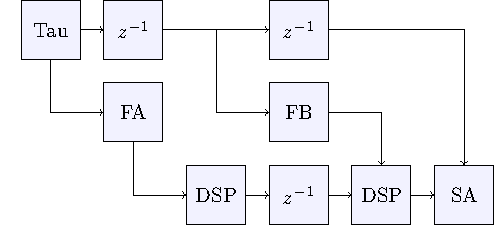
\includegraphics[scale = 1.5]{block_diagram/xcorr_diag.pdf}
	\captionof{figure}{Block diagram of pipelined calculation of cross-correlation}
	\label{fig::block_diag}
\end{figure}

The cross-correlation of two discrete signals is defined per equation \ref{eq::xcorr}.
Since only $N_{Sample}$ values are stored and available, the summation simplifies to equation \ref{eq::xcorr_ptau} for positive Taus and to \ref{eq::xcorr_ntau} for negative Taus.

\begin{align}
X_{ab}(\tau) &:= \sum_{n=-\infty}^{\infty}a\left[n\right]b\left[n+\tau\right] \label{eq::xcorr}\\
&= \sum_{n=0}^{N_{Sample}-\tau-2}a\left[n\right]b\left[n+\tau\right] \forall\tau\ge0 \label{eq::xcorr_ptau} \\
&= \sum_{n=0}^{N_{Sample}+\tau-2}a\left[n-\tau\right]b\left[n\right] \forall\tau<0 \label{eq::xcorr_ntau} \\	
\end{align}

Each time new data is available, all stored values are shifted by one storage position.
Therefore not the whole cross-correlation has to be calculated each time.
Only the newest value pair must be added and the oldest pair subtracted, resulting in two MAC-instructions per Tau and correlation.
To further improve performance, the calculation is pipelined.
Figure \ref{fig::block_diag} shows the data flow during recalculation.

\begin{itemize}
	\item Block Tau generates the actual Tau that is to be calculated.
	\item FA denotes fetch on RAM port A. It reads the corresponding cross-correlation and the (old) 	microphone values that are to multiply and subtract.	
	\item The first DSP performs $P = -(AB)+C$, with $A$ and $B$ connected to the microphone values from FA and $C$ to the cross-correlation value.
	\item FB fetches the (new) microphone values that are to multiply and add.
	\item The second DSP calculates $P = (AB)+C$, with the microphone values from FB and the prepared cross-correlation from the first DSP.
	\item Finally, SA denotes store on port A, which performs a write-back of the new calculated cross-correlation value.
\end{itemize}

Flip-flops are needed to store and shift the Taus corresponding to the single stages, as each block RAM fetch and store needs one clock cycle.
Consequently the store command comes always three clock cycles after load.
Therefore neither collision nor simultaneous read / write is possible and no collision-detection is implemented.

\section{Driver}
\label{sec::driver}

For now, the core can only be used by addressing the registers directly.
High-level access will be added in a future release.
Two low-level functions are available.
These functions are implemented as macros and should be used carefully.
Care must be taken to not confuse the microphones. 
On the PCB they are numbered from 1 to 3 but in logic the numbering goes from 0 to 2.

\begin{itemize}
	\item XCORR\_mWriteReg(BaseAddress, RegOffset, Data) \\
		Write data to the specified Register. 
	\item XCORR\_mReadReg(BaseAddress, RegOffset) \\		
		Read the content of the specified register.
\end{itemize}

\section{Test and verification}
\label{sec::test}

The core can easily be simulated by using the AXI traffic generator IP from Xilinx and feeding some well known values to the inputs.
No additional simulation files are available.
Software verification is not supported.

\section{Compatibility and License}
The core is tested under Vivado version 2016.2 and on Artix7 and Zynq7 FPGA.
The core does use hardware specific resources.
It is therefore not guaranteed to run on other FPGAs.
Since only 4 DSP slices and block RAM is used, it should run on nearly every FPGA with enough block RAM available.
However, this is not tested and may require changes to the core hdl files.
The core is supplied under no license or copyright but is the intellectual property of the authors.

\end{document}